\begin{frame}
\frametitle{Rewriting the cross entropy loss}
\begin{tikzpicture}
    [
    dot/.style = {minimum width=0.15cm,inner sep=0pt,line width=0pt,fill,circle,black,font=\small}
    ]
    \draw[] (0,4) -- (0,-1);
    \draw[] (4,0) -- (-2,0);
    \node[dot,label={0:$\w_1$}] (w1) at (2.5,1) {};
    \node[dot,label={0:$\w_2$}] (w2) at (2,2) {};
    \node[dot,label={90:$\w_4$}] (w4) at (0.25,3.75) {};
    \node[dot,label={0:$\w_3$}] (w3) at (1.25,3.5) {};
    \node[dot,label={$\w_5$}] (w5) at (-1,3) {};

    \uncover<1>{
    \draw[->,color=blue] (0,0) to (w1);
    \draw[->,color=blue] (0,0) to (w2);
    \draw[->,color=blue] (0,0) to (w3);
    \draw[->,color=blue] (0,0) to (w4);
    \draw[->,color=blue] (0,0) to (w5);

    \node[anchor=west] at (-2,-2.0) {
        \parbox{2in}{
        \small
        \begin{align*}
            \ell(U, (\x,y))
            &= 
    -\log \frac {\exp(-\trans\w_y \x)}{\sum_{j=1}^k \exp(-\trans \w_j \x)}
    \\
    \lF{\nabla_W\ell} &= \lF{W}
    \end{align*}
}};
    }

    \uncover<2>{
    \draw[->,color=red] (0,0) -- node[label={0:$\uu_2$}]{} (w2);
    \draw[->,color=red] (w2) -- node[label={0:$\uu_1$}]{} (w1);
    \draw[->,color=red] (w2) -- node[label={0:$\uu_4$}]{} (w4);
    \draw[->,color=red] (w4) -- node[label={$\uu_3$}]{} (w3);
    \draw[->,color=red] (w4) -- node[label={270:$\uu_5$}]{} (w5);

    \node[anchor=west] at (2.5,2) {
        \parbox{3in}{
        \begin{align*}
        \w_1 &= \uu_2 + \uu_1 \\
        \w_2 &= \uu_2 \\
        \w_3 &= \uu_2 + \uu_4 + \uu_3 \\
        \w_4 &= \uu_2 + \uu_4 \\
        \w_5 &= \uu_2 + \uu_4 + \uu_5 \\
        \\
        \w_j &= \sum_{i \in \ancestor(j)} \uu_i
        \end{align*}
    }
    };
    \node[anchor=west] at (-2,-2.0) {
        \parbox{2in}{
        \small
        \begin{align*}
            \ell(W, (\x,y))
            &= 
            -\log \frac {\exp(-\sum_{i\in\ancestor(y)}\trans\uu_i \x)}{\sum_{j=1}^k \exp(-\sum_{i\in\ancestor(j)}\trans\uu_i \x)}
    \\
        \lF{\nabla_U\ell} &= \lF{U} \le \lF{W}
    \end{align*}
    }};
    }

    \uncover<3>{
    \node[dot,color=darkgreen] (vC) at (0.1667,3.4167) {};
    \node[dot,color=darkgreen] (vB) at (1.75,1.5) {};
    \node[dot,color=darkgreen] (vA) at (0.75,2.0) {};

    \draw[->,color=darkgreen] (0,0) -- node[label={0:$\vv_A$}]{} (vA);
    \draw[->,color=darkgreen] (vA) -- node[label={90:$\vv_B$}]{} (vB);
    \draw[->,color=darkgreen] (vA) -- node[label={0:$\vv_C$}]{} (vC);
    \draw[->,color=darkgreen] (vB) -- node[label={270:$\vv_1$}]{} (w1);
    \draw[->,color=darkgreen] (vB) -- node[label={0:$\vv_2$}]{} (w2);
    \draw[->,color=darkgreen] (vC) -- node[label={40:$\vv_3$}]{} (w3);
    \draw[->,color=darkgreen] (vC) -- node[label={180:$\vv_4$}]{} (w4);
    \draw[->,color=darkgreen] (vC) -- node[label={270:$\vv_5$}]{} (w5);

    \node[anchor=west] at (3.25,2) {
    \parbox{3in}{
    \begin{align*}
    \w_1 &= \vv_A + \vv_B + \vv_1 \\
    \w_2 &= \vv_A + \vv_B + \vv_2 \\
    \w_3 &= \vv_A + \vv_C + \vv_2 + \vv_4 + \vv_3 \\
    \w_4 &= \vv_A + \vv_C + \vv_2 + \vv_4 \\
    \w_5 &= \vv_A + \vv_C + \vv_2 + \vv_4 + \vv_5 \\
    \\
    \w_j &= \sum_{i \in \ancestor(j)} \vv_i
    \end{align*}
}
};
    \node[anchor=west] at (-2,-2.0) {
        \parbox{2in}{
        \small
        \begin{align*}
            \ell(V, (\x,y))
            &= 
            -\log \frac {\exp(-\sum_{i\in\ancestor(y)}\trans\uu_i \x)}{\sum_{j=1}^k \exp(-\sum_{i\in\ancestor(j)}\trans\uu_i \x)}
    \\
        \lF{\nabla_V\ell} &= \lF{V} \le \lF{U} \le \lF{W}
    \end{align*}
    }};
}

\end{tikzpicture}

%\begin{align*}
%W &= (\w_1, \w_2, \w_3, \w_4, \w_5) \\
    %\color{red} U &= \color{red} (\uu_1, \uu_2, \uu_3, \uu_4, \uu_5) & \color{red} \lF{U} \le \lF{W} \\
%%V &= (\vv_A, \vv_B, \vv_C, \vv_1, \vv_2, \vv_3, \vv_4, \vv_5) & \lF{V} \le \lF{U} \le \lF{W} \\
%\end{align*}
    
\end{frame}
%%%%%%%%%%%%%%%%%%%%%%%%%%%%%%%%%%%%%%%%%%%%%%%%%%%%%%%%%%%%%%%%%%%%%%%%%%%%%%%%
\ignore{
\begin{frame}
\frametitle{U-tree}
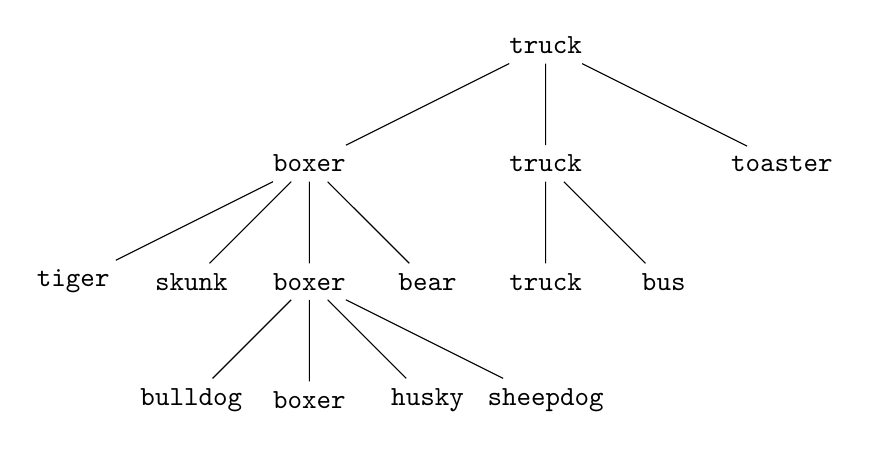
\begin{tikzpicture}
    [ level distance=1.5cm
    , level 1/.style={sibling distance=3cm}
    , level 2/.style={sibling distance=1.5cm}
    ]
\node {\texttt{truck}}
    child {node {\texttt{boxer}}
      child {node {\texttt{tiger}}}
      child {node {\texttt{skunk}}}
      child {node {\texttt{boxer}}
        child {edge from parent[draw=none]} % Added
        child {node {\texttt{bulldog}}}
        child {node {\texttt{boxer}}}
        child {node {\texttt{husky}}}
        child {node {\texttt{sheepdog}}}
      }
      child {node {\texttt{bear}}}
      child {edge from parent[draw=none]} % Added
      }
    child {node {\texttt{truck}}
      child {edge from parent[draw=none]} % Added
      child {node {\texttt{truck}}}
      child {node {\texttt{bus}}}
    }
    child {node {\texttt{toaster}}}
    ;

\end{tikzpicture}
\end{frame}
}
